\documentclass[sigconf,hyphens]{acmart}
\usepackage{graphics}

\usepackage{todonotes}
\usepackage{longtable}


% BEGIN DRAFT FLAGS
% \settopmatter{printacmref=false}
% END DRAFT FLAGS

\AtBeginDocument{%
  \providecommand\BibTeX{{%
    \normalfont B\kern-0.5em{\scshape i\kern-0.25em b}\kern-0.8em\TeX}}}


\copyrightyear{2019}
\acmYear{2019}
\acmConference[HARC '19]{Humans in the Loop: Enabling and Facilitating Research on Cloud Computing}{July 29, 2019}{Chicago, IL, USA}
 
\acmBooktitle{Humans in the Loop: Enabling and Facilitating Research on Cloud Computing (HARC '19), July 29, 2019, Chicago, IL, USA}
\acmPrice{15.00}
\acmDOI{10.1145/3355738.3355751}
\acmISBN{978-1-4503-7279-4/19/07}

%%\acmSubmissionID{123-A56-BU3}


\begin{document}

\title{Human in the Loop Virtual Machine Management on Comet}


\author{Gregor von Laszewski}
\email{laszewski@gmail.com}
\orcid{0000-0001-9558-179X}
\authornote{Corresponding author}
\author{Fugang Wang}
\email{kevinwangfg@gmail.com}
\author{Geoffrey C. Fox}
\email{gcfexchange@gmail.com}
\affiliation{%
  \institution{Indiana University}
  \streetaddress{MESH}
  \city{Bloomington}
  \state{IN}
  \postcode{47401}
}

\author{Shawn Strande}
\author{Christopher Irving}
\author{Trevor Cooper}
\author{Dmitry Mishin}
\author{Michael L. Norman}
\affiliation{%
  \institution{San Diego Supercomputer Center}
  \streetaddress{University of California, 9500 Gilman Drive}
  \city{La Jolla}
  \state{CA}
  \postcode{92093-0021}
}

\renewcommand{\shortauthors}{von Laszewski, et al.}

\newcommand{\TODO}[1]{\todo[inline]{#1}}

\begin{abstract}

  The Comet petascale system is an XSEDE resource with the goal of
  serving a large user community. The Comet project has served a large
  number of users while using traditional supercomputing as well as
  science gateways. In addition to these offerings, Comet also
  includes a non traditional virtual machine framework that allows
  users to access entire Virtual Clusters instead of just focusing on
  individual virtual machines. The virtual machine framework
  integrates a custom administration interface, a novel virtual
  machine image management back-end, industry standard hardware
  virtualization technology and leverages the Comet resource manager
  and job scheduler to provide access to Comet compute nodes. However,
  to access and manage it user input is required. In this paper, we
  summarize the efforts of human in the loop-for-cloud require as part
  of the computing activities on comet. This includes a discussion of
  how to get access, how to use the system, how to obtain support and
  what lessons we learned form the operation of this facility for
  users.

\end{abstract}

%% http://dl.acm.org/ccs.cfm.

\begin{CCSXML}
<ccs2012>
<concept>
<concept_id>10010520.10010521.10010537.10003100</concept_id>
<concept_desc>Computer systems organization~Cloud computing</concept_desc>
<concept_significance>500</concept_significance>
</concept>
<concept>
<concept_id>10011007.10010940.10010971.10011120.10003100</concept_id>
<concept_desc>Software and its engineering~Cloud computing</concept_desc>
<concept_significance>500</concept_significance>
</concept>
</ccs2012>
\end{CCSXML}

\ccsdesc[500]{Computer systems organization~Cloud computing}
\ccsdesc[500]{Software and its engineering~Cloud computing}


\keywords{cloud computing, virtual machine management}



\maketitle

\section{Introduction}\label{sec:intro}

Comet targets the \textit{long tail} of science
\cite{comet17tails}\cite{comet-vc} focusing primarily on small and
modest scale computing jobs, and those that require specialized
software environments that are not found on traditional clusters. As
such Comet has been used successfully to support science gateways,
which provide easy to use web interfaces to High Performance Computing
(HPC) systems for research communities. One strength of Comet is also
the ability to use Virtual Clusters (VCs) providing near bare-metal
performing computing resources that can be used to provision custom
software by the users to their own research teams. A key strategy that
Comet uses to serve the later community is to engage the users and
allow an interactive experience as part of a human-in-the-loop
management and usage strategy.

This strategy involves the following components requiring
human-in-the-loop actions that are targeting the workflow of a typical
interaction with the users:

\begin{description}

\item[VC Initial User Consultation.] Provides the initial consultation
  to use the VC concept of Comet.

\item[VC User Account Application.] Provides the user account to
  access the VC framework.

\item[VC Setup.] Provide the option for fully virtualized clusters
      with near zero performance overhead.

\item[VC User Training.] Employ an \textit{on-ramping} service,
which results in a fully operational software environment that
can be instantiated via the Slurm scheduler using tools
developed by the project.

\item[VC User Support.] Provides consistent user support in case
  of issues during run-time.

\end{description}

The paper is structured as follows. In Section \ref{sec:vc} we provide
a short introduction into the VC management concepts of Comet. In
Section \ref{sec:consult} we summarize our experience with our initial
user consultation. In section \ref{sec:account} we showcase our
application process followed by the VC setup in Section
\ref{sec:setup}. To effectively use the cluster we provide in Section
\ref{sec:training} our experience with user training and support. We
provide a short experience on one of the applications (Section
\ref{sec:application}. In Section \ref{sec:external} we provide
information on how to make it easier for the user to engage in
multi-cloud environments in case Comet is not suitable. We give a
conclusion in Section \ref{sec:conlusion}.

%%%%%%%%%%%%%%%%%%%%%%%%%%%%%%%%%%%%%%%%%%%%%
\section{Virtual Clusters on Comet}\label{sec:vc}
%%%%%%%%%%%%%%%%%%%%%%%%%%%%%%%%%%%%%%%%%%%%%

In \cite{comet-vc} we summarized our approach of not using common
virtualization approaches on Comet but to utilize the common queuing
system on Comet to schedule virtual machines at the same time as other
high performance computing or gateway jobs. Other frameworks may reuse
OpenStack but did not leverage the years worth of human experience
that we gathered while operating supercomputer resources with
sophisticated queuing systems within the community.

The novel Comet virtual environment is motivated by the desire to
create an efficient system architecture for virtual HPC clusters that
provides performance comparable to the underlying physical system
while at the same time leveraging the users and administrators
experience in using HPC tools and services. Hence, Virtual Clusters
that are started on Comet are running on the same servers as regular
HPC jobs. Virtual machines that constitute a VC consequently have
access to the same high-performance hardware, including the InfiniBand
interconnect via SR-IOV, local flash drives, significant amounts of
RAM and multicore CPUs with vector instruction sets \cite{comet-vc}.

The important difference to other virtualization efforts is that on
Comet we typically are not concerned with the management of a single
virtual machine, but with the management of a virtual cluster (VC)
that uses many virtual machines. Hence the concepts and needs by users
are more complex than in other virtual machine frameworks. One target
audience is the user that likes to for example test their software
stacks on a VC, another are those that can not afford to purchase
their own cluster and can through Comet obtain such a cluster for
themselves without cost. Yet another user community are those that
like to learn how to manage such clusters. The main target community
are users who have a software stack different enough from the one they
can find on typical high performance computing systems, making it
easier for them to maintain their own cluster rather than ask
administrators to install the needed software on a system not under
control by the user. Needless to say that application users with
sporadic but significant computational needs could benefit from
clusters that are specifically targeting their application software
stacks and needs.

Based on these user communities we identified a number of requirements
that we need to fulfill and have a direct impact on how to use the
system.

First, we note that the clusters on the system must be sufficiently
separable so that the clusters do not interfere with each other on the
conceptual view. Second, we like to launch multiple clusters at the
same time to share the resource on the system efficiently (see
\ref{fig:vc-view}). Third, we notice that although some application
will at one point fully automatize their software and development
stacks, an intermediate step is needed that allows the user to access
the system in an experimental fashion. This requires the easy creation
of the cluster as we like to minimize the burden on the Comet
administrators, but also the ability to integrate the management
function into the users programming frameworks. This includes not only
the ability to access it from many programming languages, but also
from the command line as one of our main users are system
administrators with sophisticated scripting background. Additionally,
we need to deliver near bare-metal experience to the users of Virtual
Clusters, thus mimicking that of a physical one, to make it attractive
for the targeted users.

\begin{figure}[htb]
    \centering
    \includegraphics[width=1.0\columnwidth]{images/vc-view.png}
    \caption{The VC architecture of comet \cite{comet-vc}}
    \label{fig:vc-view}
\end{figure}


%%%%%%%%%%%%%%%%%%%%%%%%%%%%%%%%%%%%%%%%%
\section{VC Initial User Consultation}\label{sec:consult}
%%%%%%%%%%%%%%%%%%%%%%%%%%%%%%%%%%%%%%%%%
    
One of the important aspects of Comet is a significant effort in
supporting its users. This is done through various user support teams
that focus on aspects such as gateways, traditional HPC, but most
importantly for this effort the support of Virtual Clusters. As part
of these efforts we have identified that we need to support a variety
of phases to introduce the users smoothly into obtaining their VCs
(see also Section \ref{sec:intro}).

To gain access to the advanced features of virtual cluster management
it is important that each user is vetted and an interactive interview
is carried out in which requirements and expectations are identified
and discussed. This is typically an interactive process that includes
exchange not only of a link to the documentation but an understanding
of the application needs identified between support staff and the
users.

The important part to note is that the funding for Comet does not
project the education of what users do with their Virtual Clusters,
but a level of sophistication is required by the users so that the
operators of Comet can be confident that the users know what they are
doing. Within the project we refer to this check casually as,
\textit{a user must be that tall to use a VC}. As part of this we must
be assured that the user have minimal understanding of system
administration and security to make sure the cluster stay up to date
and does not pose a security risk. Due to this assumption, we do not
spend too much effort on educating users to administer their
cluster(s). We found this user vetting process necessary as in
contrast to commercial clouds no monetary value is provided that gives
incentives to make sure exploits to the deployed cluster is not wide
spread. This is one of the most important distinction between Comets
(or other academic clouds) and commercial clouds. Hence we provide a
short interview with the team to analyze their requirements, but also
to analyze their expertise. If either is a limitation to the user of
Virtual Clusters the user will be referred to other resources that may
be more suitable. Through this needed requirements, the overall user
community for Virtual Clusters has been traditionally small but
sophisticated.

%%%%%%%%%%%%%%%%%%%%%%%%%%%%%%%%%%%%%%%%%
\section{Account Management}\label{sec:account}
%%%%%%%%%%%%%%%%%%%%%%%%%%%%%%%%%%%%%%%%%

Once it is identified that the project is suitable, an account request
is issued that follows best practices established at SDSC and NSF
sponsored projects. This process is also integrated with the XSEDE
allocations process. It requires necessary interaction and can not be
fully automatized due to the access rights a user obtains on Comet.
The process is documented in Figure \label{fig:account}.

\begin{figure}[h]
  \centering
  \includegraphics[width=\linewidth]{images/commet-account-creation.png}
  \caption{Comet account process.}\label{fig:account}
  \Description{Comet account process.}
\end{figure}

As we value security, access to the management machine that governs
Virtual Cluster activities by the user is protected through 2-factor
authentication with a YubiKey. This key is issued by Comet and send to
the user with postal mail. Although, the sending of the YubiKey
increases wait time, it is possible to send it via express mail making
it a very short waiting period. The application to obtain an XSEDE
allocation takes typically longer, so submission of the key is not an
issue. It is impoartant to recognize that even, commercial
organizations such as Google have recently also adopted the use of
YubiKeys, so we are well ahead of the trend. After the account is
deactivated the user is expected to return the YubiKey. Due to the
minimal cost of the keys the use of YubiKeys does not put an
extraneous burden on the overall operational costs. Even if a user
were to misplace the key, or the key would break, a quick replacement
could be provided within one day.

%%%%%%%%%%%%%%%%%%%%%%%%%%%%%%%%%%%%%%%%%
\section{Virtual Cluster Setup}\label{sec:setup}
%%%%%%%%%%%%%%%%%%%%%%%%%%%%%%%%%%%%%%%%%

As part of the user experience we educate the users to manage their
own VC. The way a VC is set up is to give the users access to a
management interface on a special management node on Comet that allows
the users to manage their clusters from this node. The YubiKey is used
for authentication and the user is added to the authorized users
during the account creation process.

The important aspect here is that we do not use the same virtual
machine management framework as commercial clouds or academic clouds
using OpenStack. Instead we have a much easier interface that manages
the entire cluster. This interface has been introduced in
\cite{comet-vc}. It contains a REST API, but also a command line
client. The software used to access this interfaces via the command
line is called cloudmesh and is available as an open source project
\cite{cloudmesh-comet-manual}. It is very easy to use and the user can
within their assigned cluster, add and remove nodes to address
on-demand needs. The clusters can be shutdown or started with a simple
command so that users can save their XSEDE allocations and use them
only if this resource is used. Limitations on the cluster size and
usage can be set by the administrative staff of Comet. Very important
is that the Virtual Clusters can leverage the underlying InfiniBand
network. Due to this simple interface either as command line or as
REST interface the management of the VC is rather simple and can be
accomplished even by non experts.

%%%%%%%%%%%%%%%%%%%%%%%%%%%%%%%%%%%%%%%%%
\section{Virtual Cluster User Training and Usage}\label{sec:training}
%%%%%%%%%%%%%%%%%%%%%%%%%%%%%%%%%%%%%%%%%

Early on we realized that the on-ramp in using Comet must be small and
that those that manage Virtual Clusters should be able to do so with
ease. The creation of the cloudmesh tool to interface with the
clusters and manage them made it possible to reduce the effort it
takes for training users to use the VC technology. We provided an easy
manual page and especially the cloudmesh extensible command shell
allows users to manage their clusters with ease. Behind the scene
cloudmesh communicates with a REST service called Nucleus that
interfaces directly with the Comet resource manager and job queuing
system. However all of this is hidden form the user who has the
experience of obtaining direct access to the system. Tutorials given
at XSEDE, PEARC and a presentation at NIST added to the dissemination
activities.

%%%%%%%%%%%%%%%%%%%%%%%%%%%%%%%%%%%%%%%%%
\section{Virtual Cluster User Support} \label{sec:support}
%%%%%%%%%%%%%%%%%%%%%%%%%%%%%%%%%%%%%%%%%

The user support we provide is limited to the management of VCs. It is
not targeting to educate users to become a system administrator. As we
see in the discussion this has been the biggest challenge with our
approach. E.g. our technology is sound and easy to use, but once the
cluster is available we found unexpected challenges caused by the
users using and managing such clusters.


%%%%%%%%%%%%%%%%%%%%%%%%%%%%%%%%%%%%%%%%%
\section{Towards General Interactive NIST Virtual Clusters}\label{sec:vc-nist}
%%%%%%%%%%%%%%%%%%%%%%%%%%%%%%%%%%%%%%%%%

Although the VC software we defined is easy to use we worked together
with NIST and identified that lessons learned from the Comet
experience could in general benefit the NIST community as part of the
Big Data Reference Architecture Interface Definition
\cite{www-vol8-v3}. As such we have developed a new specification that
leverages our earlier work on Comet \cite{comet-vc}.

A Virtual Cluster is modeled as manager node, and one or more compute
nodes. The manager node usually serves as a login node and can be
accessed from outside via a public IP. The compute nodes are connected
to the manager node via a private, usually high performance (high
throughput and low latency) network and thus accessible only from the
manager node. To use the VC, login to the manager node, and from there
one can login to any compute node, or submit a job to run on the
compute nodes. The resources of the cluster are depicted in Tables
\ref{tab:vc}, \ref{tab:node}, and \ref{tab:nic}. The path of the REST
framework are showcased in \ref{tab:path}. Although not funded by
Comet, it is important to note that the interaction with NIST is an
important human lead activity by the developers of the Comet VC
software. It allows to reciprocally disseminate experiences between
two communities. This enables us to bring this feedback from NIST back
to the Comet team. Hence, we indirectly extended the user community
beyond Comet. Most importantly it has lead the a document submitted to
NIST describing the specification of Virtual Clusters
\cite{www-vol8-v3}.


\begin{table}

\caption{Virtual Cluster Resource \cite{nist-virtual-cluster-spec}}\label{tab:vc}
\begin{tabular}{p{0.2\columnwidth}p{0.2\columnwidth}p{0.5\columnwidth}}
\toprule
Property & Type & Description\\
\midrule
name & string & The name of the VC\\
description & string & A description of the virtual
cluster\\
owner & string & Username of the owner of the virtual
cluster\\
manager & \protect\hyperlink{node}{Node} & Manager node of the virtual
cluster\\
nodes & array{[}Node{]} & List of nodes of the virtual
cluster\\
\bottomrule
\end{tabular}

\bigskip
\caption{Node Resource \cite{nist-node-spec}}\label{tab:node}

\begin{tabular}{p{0.2\columnwidth}p{0.2\columnwidth}p{0.5\columnwidth}}
\toprule
Property & Type & Description\\
\midrule
name & string & Name of the node\\
state & string & Power state of the node\\
ncpu & integer & Number of virtual CPUs of the node\\
ram & string & RAM size of the node\\
disk & string & Disk size of the node\\
nics & array{[}NIC{]} & List of network interfaces of the
node\\
\bottomrule
\end{tabular}

\bigskip
\caption{Network Interface Card Resource \cite{nist-nic-spec}}\label{tab:nic}

\begin{tabular}{p{0.2\columnwidth}p{0.2\columnwidth}p{0.5\columnwidth}}
\toprule
Property & Type & Description\\
\midrule
mac & string & MAC address of the node\\
ip & string & IP address of the node\\
\bottomrule
\end{tabular}
\end{table}


\begin{table}
\caption{Path of the Virtual Cluster}\label{tab:path}
\begin{tabular}{p{0.08\columnwidth}p{0.45\columnwidth}p{0.37\columnwidth}}
\toprule
HTTP & Path & Summary \\
\midrule
get & /virtualcluster & Returns a list of Virtual Clusters \\
get & /virtualcluster/\{name\} & Returns the named VC \\
put & /virtualcluster/\{name\} & Uploads an VC to the list of  Virtual Clusters\\
delete & /virtualcluster/\{name\} & Deletes the named VC \\
get & /virtualcluster/\{name\}/\{node\} & Node of the named VC\\
put & /virtualcluster/\{name\}/\{node\} & Updates or adds a node to the VC\\
delete & /virtualcluster/\{name\}/\{node\} & Delete a node in the VC\\
\bottomrule
\end{tabular}
\end{table}


\section{Virtual Cluster Monitoring}

As we use the common queuing system that is bound into XSEDE
resources, we can therefore reuse the monitoring and auditing
infrastructure available as part of XSEDE. This includes XDMoD
\cite{tas-view}. We showcase in Figure \label{fig:usage} a graph of
projects and their number of jobs (a job is a cluster invocation) used
as part of the allocations these projects have received.

\begin{figure*}[h]
  \centering
  \includegraphics[width=\linewidth]{images/xdmod_Comet_VC_Jobs_Usage_2016-01-01_to_2018-12-31.png}
  \caption{Comet usage.}\label{fig:usage}
  \Description{Comet usage.}
\end{figure*}

Due to the interaction to obtain a VC users may desire to gain access
to the clusters quickly. The result is showcased in Figures
\ref{fig:wait1}, \ref{fig:wait2}, and \ref{fig:wait3}.


We conducted a wait time analysis with all VC jobs data including over
23k records. Please note that each VC job here corresponds to a
request of starting one or more compute nodes as part of a specific
virtual cluster. Thus the wait time is equivalent to the time a user
has to wait for the compute node(s) to start after she or he requested
to start the VC node(s). Figure \ref{fig:wait1} shows the wait time in
minutes for the VC jobs in their submitted order. We can see from the
figure that other than a small percentage, which were related to
resource requirements not met, or an error in the back-end that
required human intervention, most other jobs fulfilled the user
requests in a very timely fashion. Figure \ref{fig:wait2} shows the
empirical cumulative distribution of the job wait time. We can see
from the figure that 3 quarters of the jobs waited under 12.3 minutes,
while 90\% waited less than 76.9 minutes. Figure \ref{fig:wait3} shows
the same distribution but was in log scale for the x axis, for a more
clear view of the lower end. E.g., this helps to show that about half
of the jobs waited only about 1 minute. Please note that after the
cluster is provisioned the nodes are readily available. It it is
obvious that setting up a cluster and reserving nodes is much less
time consuming than going through a procurement process to obtain a
hardware based cluster.

\begin{figure}[h]
  \centering
  \includegraphics[width=\linewidth]{images/vc_waittime_sum1.pdf}
  \caption{Comet wait time.}\label{fig:wait1}
  \Description{Comet wait time.}

\end{figure}

\begin{figure}[h]
  \centering

  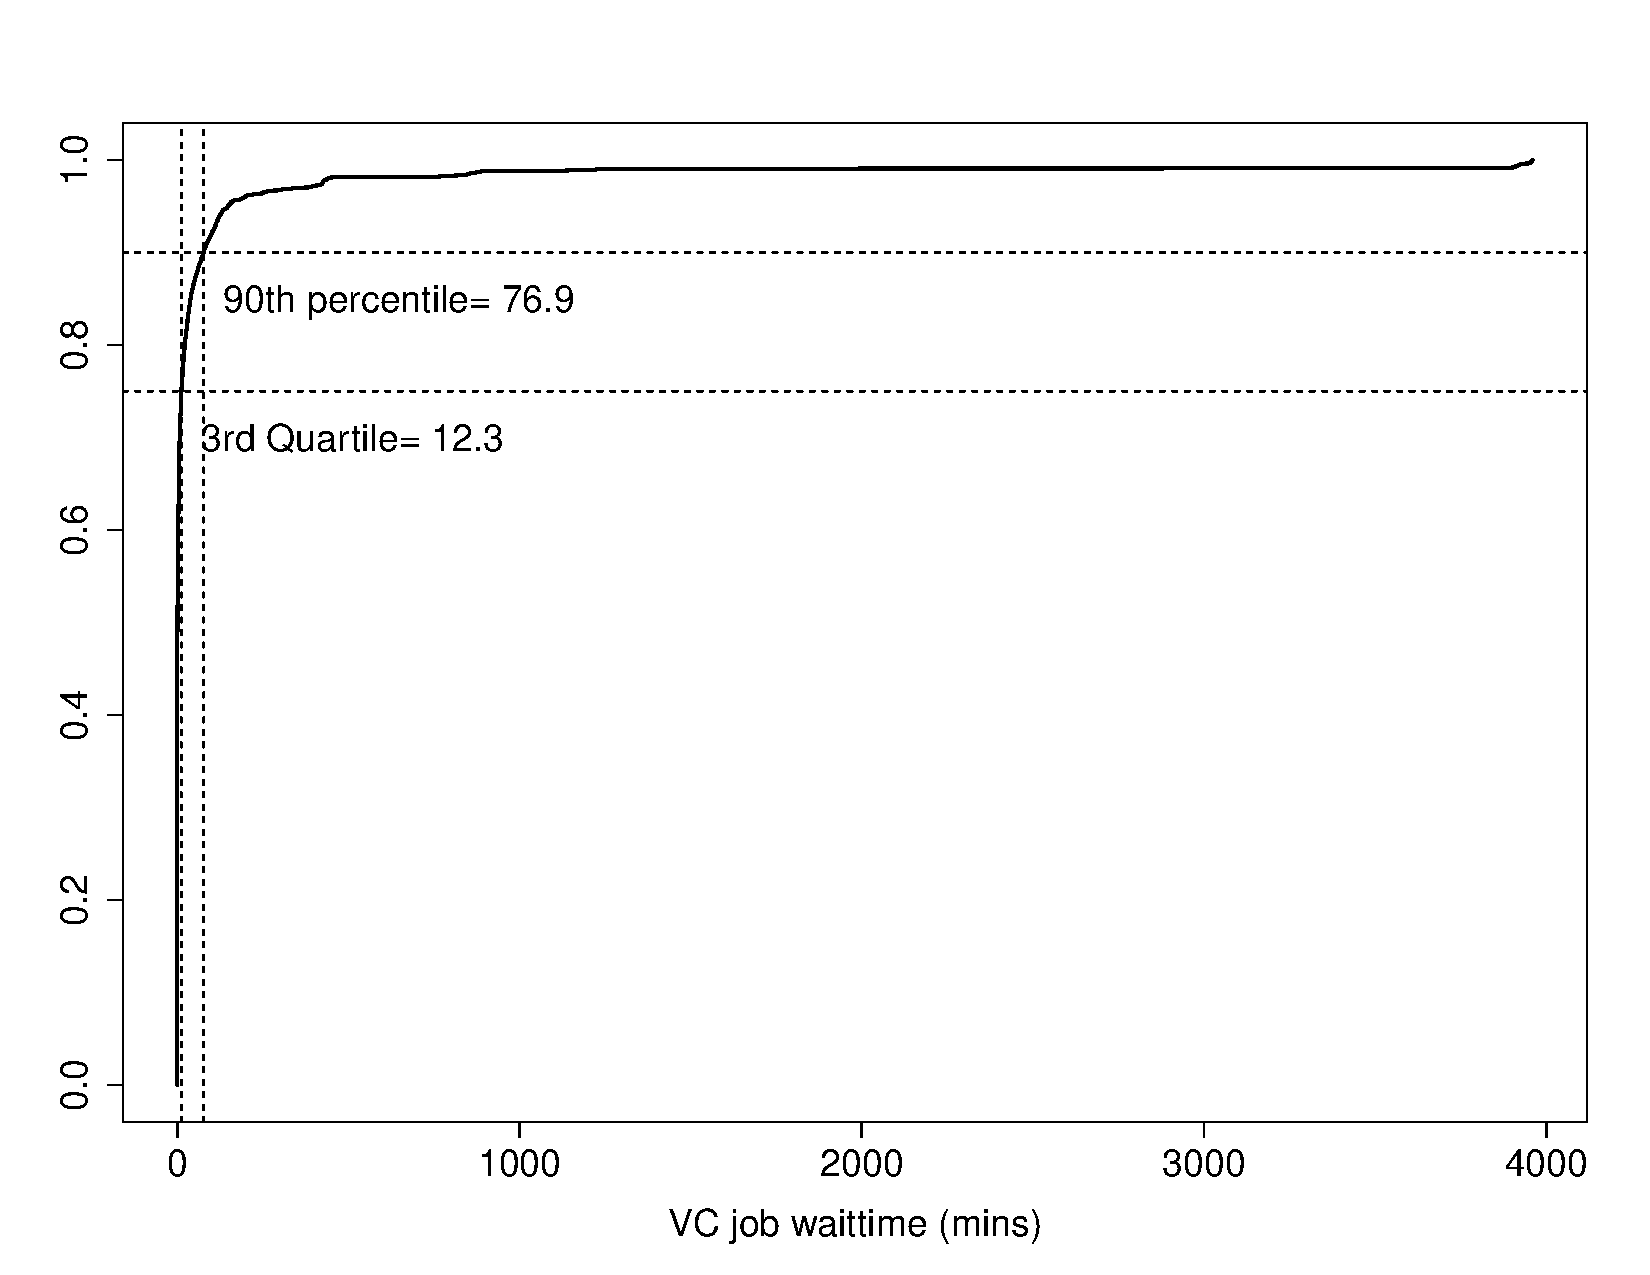
\includegraphics[width=\linewidth]{images/vc_waittime_sum2.pdf}
  \caption{Comet wait time.}\label{fig:wait2}
  \Description{Comet wait time.}

\end{figure}

\begin{figure}[h]
  \centering

  \includegraphics[width=\linewidth]{images/vc_waittime_sum3.pdf}
  \caption{Comet wait time.}\label{fig:wait3}
  \Description{Comet wait time.}

\end{figure}


\section{Application Integration}\label{sec:application}

Virtual Clusters have been applied to a number of applications. This
includes the list of applications listed in Table \ref{tab:apps}.
Requests include different application requirements. This entails
education, custom software stacks, replication of existing cluster
environments, isolation of cluster environments for security reasons,
as well as experimenting of inclusion of more compute resources for
application domains. In all cases the users were cluster experts.

We have been contacted however by other application users and if the
project was not appropriate, we referred them to other XSEDE or cloud
resources. Hence, we limited our access to the most advanced user
communities.

\begin{table*}

\caption{Virtual Cluster Applications}\label{tab:apps}

\begin{tabular}{ll}
%{p{0.2\columnwidth}p{0.7\columnwidth}}
\toprule
Name & Description\\
\midrule
LIGO & Cluster that integrates in OSG for detection of gravity waves \\
PRAGMA & Virtual Clusters for Environmental Science \\
OSG & Portal to VC Resources \\
Benchmark & Benchmarking petaflop HPC algorithms weather, CFD, and others \\
BigData & VC for evaluation for NIST \\
Darknets & Virtual Clusters for the analysis of darknets \\
THMC & 3D Thermal-Hydrologic-Mechanical-Chemical \\
Performance & tools to capture and analyze memory activities in applications\\
LIDAR & high resolution topography data \\
Biology & Genomic data analysis software stack \\
Astrophysics & HPC-specific workflows for simulating events necessary for precision astrophysical measurements \\
CMS & resources to process 800 Million simulated proton proton
collisions in the CMS detector \\
Lifemapper & a high-throughput species distribution (range)
modeling system and the main computational platform \\
Education & Campus champion clusters for universities \\ 
\bottomrule
\end{tabular}

\end{table*}

\section{Integration of External Services}\label{sec:external}

In case we found out that other clouds are more appropriate, cloudmesh provides a very easy multi-cloud interface in addition to its comet virtual cluster interface. This is possible through templated virtual machine management for the different clouds.

Hence it is possible to start a VM on a cloud and log into it with three simple commands:

\begin{verbatim}
    $ cms set cloud=aws 
    $ cms vm boot
    $ cms vm ssh
\end{verbatim}

In case we like to use a different cloud all we have to do is to set and boot a vm on that cloud such as:

\begin{verbatim}
    $ cms set cloud=azure 
    $ cms vm boot
    $ cms vm ssh
\end{verbatim}

To document these features we provide online documentation
\cite{www-cloudmesh-manual,las-cloudmesh}, but also have developed an
ePub and PDF book creation tool called {\em cyberaide-bookamanger}
\cite{las-bookmanager}, allowing us to custom design manual
particularly suited for a specific topic or user needs and interests.
This project is also used at Indiana University to manage over 2000
pages of educational material for several classes related to cloud
computing engineering \cite{las-cloud,las-python} and big data
\cite{las-bigdata-class}.

\section{Conclusions and Lessons Learned}\label{sec:conclusion}

Although our project delivered a unique and superb software stack
allowing users and resource providers to utilize VCs with ease by the
humans-in-the-loop, we found that the most limiting factor in using
this resource were not only limitations projected by the user
community, but also by a shift of priorities within the user
community.

Comet was a one of the earliest cloud resources publicly offered to
the XSEDE user community. However, it used the non traditional
abstraction of a VC instead of just virtual machines. While most in
the community desired to get a grasp about how to leverage virtual
machines Comet bypassed this step and pioneered Virtual Clusters. As
many in the community including educational activities solely focused
on efforts such as OpenStack, while trying to leverage the community
development efforts, many such clouds had to find out that managing
such a cloud is very time consuming and is most effectively done while
not sharing the infrastructures with others but dedicate the entire
cluster to OpenStack. We operated both environments and found that the
effort to manage the Comet VC framework was smaller than that of
managing OpenStack. This is naturally also motivated by the fact that
the maintenance conducted by the human administrators were also
covering the regular HPC and gateway efforts, as we run both at the
same time and leverage existing queuing systems.

In addition, we recently saw a shift in interest by many in the
community away from virtual machines and instead towards the adoption
of containers. Not surprisingly, the appearance of Kubernetes as a
cluster management tool for containers can be seen as an adoption of
the vision that we already projected in Comet: {\em That of using
  Virtual Clusters}. However, instead of using virtual machines such
as we have used in Comet nowadays containers as part of Kubernetes has
become most popular.

While talking to many as part of our activities we identified out some
aspects that are out of our control. Although we provided a very good
framework, we had difficulties with some users due to the reason that
they were not sufficiently versed to manage their own cluster stacks.
In addition we also saw that user sustainability was an issue as some
users left the team that was investigating Comet as a resource or
suddenly had different priorities not allowing them to continue with
their planed projects. In one instance we even had a team that due to
obtaining their own hardware (although less powerful) was no longer in
the position to use Comet as they only had time to support their own
cluster.

However, at this time the biggest impact will be the use of
Kubernetes. As a remedy we see that pre-made software stacks
especially the deployment of Kubernetes clusters could provide a
solution to this human-in-the-loop dilemma. It will naturally not
completely automatized and still requires the involvement of the user.

Also leveraging the VC capabilities Comet by sysadmins might help
bursting other Kubernetes clusters to Comet virtual machines. Adding
Kubernetes as a platform within virtual clusters is a desirable goal.

\begin{acks}

  Comet is supported by NSF grant: ACI \#1341698 Gateways to
  Discovery: Cyberinfrastructure for the Long Tail of Science.

\end{acks}

\bibliographystyle{ACM-Reference-Format}
\bibliography{references}

\end{document}

https://www.overleaf.com/project/5d14cc89d0a9e82a51d171ea


%refs to be included:

%\cite{las18impact}
%\cite{las14impact}

